%Tok povrchem krychle. Gaussova věta
\documentclass{standalone}
\usepackage{tikz}
\usetikzlibrary{intersections, calc}
\usepackage{tikz-3dplot}


\begin{document}
  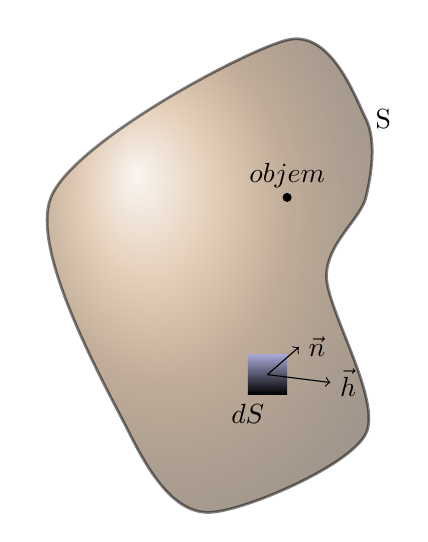
\begin{tikzpicture}
      \coordinate (dS) at (1.5,0.5);
      \shade[ball color=gray!10!brown,opacity=0.50,line width=1,draw=black] plot [smooth cycle]
        coordinates {(0,0) (1,-1) (3,0) (2.5,2) (3,3) (3,4) (2,5) (-1,3) };
      \draw (3,4) node[right]{S};
      % ploska dS
      \shade[bottom color=black,top color=black!50!blue!35](dS)
        node[below]{$dS$} rectangle +(0.5,0.5);
      \draw[->] (dS) ++ (0.25,0.25) -- +(0.4,0.35) node[right]{$\vec{n}$};
      \draw[->] (dS) ++ (0.25,0.25) -- +(0.8,-0.1) node[right]{$\vec{h}$};
      \draw[fill=black] (2,3) circle (0.05) node[above, black]{$objem$};
  \end{tikzpicture}
\end{document}